\documentclass[output=paper]{langscibook} 
\author{Laura J. Downing\lastand Morgan Nilsson\affiliation{University of Gothenburg, Sweden}}
\title{Prosodic restructuring in Somali nominal constructions}

% \chapterDOI{} %will be filled in at production
 
\abstract{This paper investigates variability in the realization of High tones in some nominal constructions of Somali. Previous work on Somali tone suggests that most determiners and all nominal modifiers should realize a High tone when they combine with the noun they modify. However, our study finds that there is considerable variability in the realization of High tones on nominal determiners and modifiers, with the High tone often not realized. This phenomenon of variability in tone realization is quite reminiscent of Swedish, which shares with Somali the property that tone realization is culminative within some prosodic domain. Recent work on Swedish has argued that variable non-realization of High tone is best analyzed as prosodic restructuring: reducing the number of culminative tonal domains in a construction necessarily leads to a reduction in the number of surface High tones. We argue that prosodic domain restructuring also provides the most plausible analysis of High tone reduction in Somali nominals.}

\begin{document} 
\maketitle
% \textbf{Keywords:} tone, Swedish, culminativity, determiners, nominal modifiers


\section{Introduction}
\label{sec:downing:1}
It is uncontroversial that the Somali tonal system has canonical stress-like properties, as defined in \cite{Downing2010} and \citet{Hyman2006,Hyman2011,Hyman2012,Hyman2014}. Work by \citet{Hyman1981,Hyman2006,Hyman2012,LeGac2003,Green2016}, and \citet{Saeed2004} agrees that High tone is \textit{culminative}: no more than one High tone can occur per (minimal Phonological) Word (PWord). The position of High tones is, roughly, \textit{demarcative}: they occur on either the penult or final mora of a PWord. Only some proper names have a High tone in another position \citep[22]{Saeed1999}. How to account for these generalizations, which hold for PWords in isolation, is more controversial. Some possibilities are: underlying accent \citep{Banti1988,Green2016,LeGac2003}, (underlying) High tone \citep{Andrzejewski1964,Andrzejewski1979,Andrzejewski1981,Armstrong1934,Hyman2006,Hyman2014,LeGac2016}, or no underlying tone or accent, rather surface tone is the result of morphological tone\slash accent assignment principles (\citealt{Hyman1981,Mous2009}). Addressing this problem in detail is outside the scope of this particular paper. However, we do assume that Somali is a tonal language, not an (underlyingly) accentual one.

The goals of our investigation are twofold: to document the realization of High tones in some nominal constructions, and to account for the position and number of High tones that occur within these constructions in terms of matches and mismatches between morphosyntactic structure and prosodic structure.\footnote{We adopt the approach to defining mismatches between morphosyntactic and prosodic structure developed in work like: \citet{Downing1999,Downing2016,Inkelas1993,inkelas2014interplay,Ito2012,Ito2013,Nespor1986,Riad2012,Selkirk1986,selkirk2011syntax,Vigário2010}, and \citet{vogel2010phonology}. See \citet{Green2016} for a recent alternative analysis of Somali prosody within this general framework.} The central empirical finding of the paper is presented in \sectref{sec:downing:2}, which shows that a number of Somali nominal constructions in our corpus do not have the tone pattern expected from the previous literature because the expected High tone on the determiner or modifier is ``missing''. In  \sectref{sec:downing:3}, we argue that familiar tone or intonation processes like the Obligatory Contour Principle (OCP) or Final Lowering do not plausibly account for the missing High tones. In  \sectref{sec:downing:4}, we propose that prosodic restructuring provides a better account: a reduction in the number of prosodic domains a construction is parsed into leads to a reduction in the number of High tones that can be realized in the construction when High tone is a culminative property of the domain. We draw a parallel between the prosodic restructuring found in Somali and the prosodic adjunction processes that have been proposed by \citet{Myrberg2015} and \citet{Riad2016} for Swedish, a language with a surprising number of prosodic properties in common with Somali.


\section{Data to be accounted for}
\label{sec:downing:2}

This paper presents preliminary results of a study of the prosody of some nominal constructions of Somali, based on recently collected elicitation data. We begin by summarizing the sources of High tones expected in nominal constructions for the data we investigated. Then we present the tone patterns attested in our data and give more information about our corpus.


\subsection{Expected High tones in (non-subject) nominal constructions from the literature}


\citet{Hyman1981,Saeed1993,Saeed1999} and \citet{Green2016} show that all Somali nouns in isolation have a High tone on either the penult or the final mora. That is, High tone is obligatory in certain morphosyntactic constructions. The position is determined by morphological factors (e.g., declension class; ``gender''; singular vs. plural), not phonological factors. We give a few examples in \REF{ex:downing:1}; note that compounds have a single High tone, on either the penult or the final mora:
 
\ea  Somali nominals \label{ex:downing:1}
  \ea tonal minimal pairs \label{ex:downing:1a}
  
  \glll
  \textit{ínan} ~ \textup{‘boy’} \hspace{1cm} vs.  \hspace{1cm}   \textit{inán}   ~ \textup{‘girl’}\\
  \textit{béer}  ~ \textup{‘liver’} \hspace{1cm}  vs. \hspace{1cm} \textit{beér} ~ \textup{‘garden’}\\
  \textit{éy} ~ \textup{‘dog’} \hspace{1cm}  vs. \hspace{1cm}   \textit{eý} ~ \textup{‘dogs’}\\
  
  \ex tone on penult vs. ultima in phonologically analogous words\label{ex:downing:1b}
  
  \begin{tabbing}
  sonkór~~ \= \textup{‘house’}\kill
  \textit{dukáan} \> \textup{‘shop’}\\
  \textit{caleén} \> \textup{‘leaf’}\\
  \textit{sonkór} \> \textup{‘sugar’}\\
  \textit{kibís} \> \textup{‘bread’}\\
  \textit{súbag} \> \textup{‘butter’}\\
  \textit{mindí} \> \textup{‘knife’}\\
  \textit{gúri} \> \textup{‘house’}
  \end{tabbing}

  \ex compounds \label{ex:downing:1c}

  \textit{dayaxgacméed} \textup{‘satellite’ (cf.} \textit{dáyax} \textup{‘moon’;}  \textit{gacmeéd} \textup{‘of hands’)}\\
  \textit{lacagháye} \textup{‘cashier’    (cf.}   \textit{lacág} \textup{‘money’;} \textit{hay-} \textup{‘have, hold’;} \textit{-e} \textup{agentive)}\\
  \textit{caanagéel} \textup{‘camel milk’ (cf.}   \textit{caanó} \textup{‘milk’;}  \textit{géel} \textup{‘camels’)}\\
  \textit{madaxweýne} \textup{‘president’ (cf.}   \textit{mádax} \textup{‘head’;}  \textit{wéyn} \textup{‘big’)}\\
  \z
\z

Nouns can be followed by a number of determiners. As shown in the list in \REF{ex:downing:2}, while the definite determiner is toneless, the other determiners introduce a High tone:\footnote{The \textit{\textbf{k}/g/h/Ø} vs. \textit{\textbf{t}/d/sh} alternations in the Somali determiner system illustrated in our data is conditioned by gender agreement: masculine nouns take the \textit{k/g/h/Ø} series of determiners, while feminine nouns take the \textit{t/d/sh} series. The allomorphy found in both series of determiners is phonologically conditioned. See, e.g., \citet{Saeed1993,Saeed1999}, for detailed discussion of this sandhi phenomenon.}


\noindent\parbox{\textwidth}{\ea  Somali determiner types \citep[111--117]{Saeed1999} \label{ex:downing:2}
  \ea {Definite    \textit{-ka/-ta}}\\
  \ex  {Remote definite  \textit{-kií/-tií}}\\
  \ex  {Interrogative    \textit{-keé/-teé}} `which'\\
  \ex  {Possessives  \textit{-káyga/-táyda} ‘my’, \textit{-káaga/-táada} ‘your (sg.)’,           \textit{-kíisa/-tíisa} ‘his’, \textit{-kéeda/-téeda} ‘her’, \textit{-kayága/-tayáda} ‘our (excl.)’, \textit{-kéenna/-téenna} ‘our (incl.)’, \textit{-kíinna/-tíinna} ‘your (pl.)’, \textit{-kóoda/-tóoda} ‘their’}\\
  \ex  {Demonstrative  \textit{-kán/-tán} `this', \textit{-kaás/-taás} `that'}\\
  \z
\z}

According to work like \citet{Green2016,Hyman1981}, and \citet{Saeed1993,Saeed1999}, when the High-toned determiners occur in combination with a noun, they retain their High tone, as illustrated in \REF{ex:downing:3}. While \citet[191]{Hyman1981} mentions a process of accent (High tone) reduction on possessive determiners following a noun, only an example or two is provided. None of the determiners change the tone of the base noun, except \textit{{}-keé/-teé} ‘which?’ (\ref{ex:downing:3h}, \ref{ex:downing:3i}).


\ea  Somali nouns with determiners \citep[160--168]{Saeed1993} \label{ex:downing:3}
  \ea  \textit{nín}   ‘man’  |  \textit{nín-ka}   ‘the man’\label{ex:downing:3a}\\
  \ex  \textit{naág}  ‘woman’ |  \textit{naág-ta}  ‘the woman’ \label{ex:downing:3b}\\
  \ex  \textit{nín}  ‘man’  | \textit{nín-kán}  ‘this man’\label{ex:downing:3c}\\
  \ex  \textit{naág}  ‘woman’ |  \textit{naág-tán}  ‘this woman’\label{ex:downing:3d}\\
  \ex  \textit{sáddex}  ‘three’ | \textit{sáddex-daás}   ‘those three’\label{ex:downing:3e}\\
  \ex  \textit{shúqul}  ‘work’ | \textit{shúqul-káyga}  ‘my work’\label{ex:downing:3f}\\
  \ex  \textit{lacág} ‘money’ | \textit{lacág-táada} ‘your money’\label{ex:downing:3g}\\
  \ex  \textit{nín}  ‘man’  | \textit{nin-keé}  ‘which man?’\label{ex:downing:3h}\\
  \ex  \textit{naág} ‘woman’ | \textit{naag-teé} ‘which woman?’\label{ex:downing:3i}\\
  \z
\z
 
\citet{Green2016,Hyman1981}, and \citet{Saeed1993} observe that the modifier in a Noun+modifier phrase – Noun+Noun or Noun+Adjective – is also expected to be realized with a High tone when the phrases are pronounced in isolation.\footnote{Noun+Noun (N+N) modifier phrases are called ``genitive constructions'' by \citet{Hyman1981} and \citet{Saeed1993}. \citet{Green2016} refer to N+N modifier phrases as ``associative constructions'' and, following \citet{Saeed1993}, use the term ``attributive adjective'' for the Noun+adjective construction. See \citet{Saeed1993} for detailed discussion of Noun+modifier constructions in Somali.} This is illustrated in \REF{ex:downing:4}, where we see that a High tone is assigned to the final vowel of the (indefinite) postnominal modifier, while the modified noun keeps its base High tone pattern.\footnote{Only a few adjectives, e.g., \textit{dhéer} ‘long’, \textit{wéyn} ‘big’ \citep[105--106]{Saeed1999}, and some female proper names seem to constitute exceptions to the generalization that modifiers in Noun+modifier phrases have a High tone on the final mora.} Note that numbers are considered nouns \citep[123]{Saeed1993} and can head Noun+modifier phrases, as shown in (\ref{ex:downing:4b}, \ref{ex:downing:4c}).


\ea  Somali Noun+modifier phrases (\citealt{Hyman1981,Green2016}; our elicitation notes)  \label{ex:downing:4}
  \ea \textit{géed} \textit{wiíl}  ‘a tree of a boy’  (cf. \textit{wíil} ‘boy’) \label{ex:downing:4a}\\
  \ex \textit{áfar} \textit{buúg}  ‘four books’  (cf. \textit{búug} ‘book’)\label{ex:downing:4b}\\
  \ex \textit{labó} \textit{sabuurad-oód}  ‘two blackboards’  (cf. \textit{sabuurád} ‘blackboard’)\label{ex:downing:4c}\\
  \ex \textit{gacán-ta} \textit{midíg}  ‘the right hand’  (cf. \textit{mídig} ‘right side’)\label{ex:downing:4d}\\
  \ex \textit{mindí-da} \textit{Maxaméd}  ‘the knife of Maxamed’  (cf. \textit{Maxámed})\label{ex:downing:4e}\\
  \ex \textit{gaarí} \textit{cusúb}  ‘a new car’\label{ex:downing:4f}\\
  \ex \textit{shúqul} \textit{adág}  ‘hard work’\label{ex:downing:4g}\\
  \z
\z
 
In sum, many nominal constructions are expected to have two High tones: one on the noun and one on the following determiner or modifier (noun or adjective).

In keeping with the one High tone per Prosodic Word (PWord) principle, \citet{Green2016} propose that Noun+determiner (H-toned) and Noun+modifier constructions have the same prosodic representation: namely, they are both parsed as independent PWords from the noun they modify. The representations in \REF{ex:downing:5} adapt \citegen{Green2016} analysis by abstracting away from the PWord-min vs. PWord-max distinction they argue for; surface High-toned morphemes are \textbf{bolded}:


\ea  Prosodic structures for Somali nominals; parentheses indicate PWords (adapting \citealt{Green2016})  \label{ex:downing:5}
\ea  N+definite  (\textbf{N})\textsubscript{PWord} def\label{ex:downing:5a}\\
\ex  N+H-toned determiner  (\textbf{N})\textsubscript{PWord} (\textbf{Det})\textsubscript{PWord}\label{ex:downing:5b}\\
\ex  compound  ((N) (\textbf{N}))\textsubscript{PWord}\label{ex:downing:5c}\\
\ex  N+modifier  (\textbf{N})\textsubscript{PWord} (\textbf{Modif})\textsubscript{PWord}\label{ex:downing:5d}\\
\z
\z

Notice the parallelism in the structure of N+determiner (\ref{ex:downing:5b}) and N+modifier (\ref{ex:downing:5d}). These representations form the starting point for our investigation.


\subsection{Our data}

The new data discussed in this paper were collected in 2016 through elicitation at the University of Gothenburg, working mainly with one speaker from Kismayo and two speakers from Mogadishu. The overall corpus comprises 10,002 individual utterances (tokens) representing 2,970 different types. The NPs were provided both in isolation and in short sentences, in morphosyntactic contexts where the variable High tone is expected to consistently occur.

What we find in these data is that the nominal constructions in (\ref{ex:downing:5b}) and (\ref{ex:downing:5d}) do not consistently have the High tone patterns expected from previous work on Somali prosody. Instead, the High tone on the determiner or nominal modifier is often ``missing''. For example, the possessive determiner is seldom realized with its expected High tone. Out of a total of 1,068 instances of N+possessive constructions in our corpus,\footnote{This set of 1,068 excludes constructions containing the shorter (indefinite) possessive suffixes, in which tonal differences reflect the distinction between a non-focused subject and other syntactic functions.} 929 (87\%) do not realize a High tone on the possessive suffix. This is illustrated in \REF{ex:downing:6}. 


\ea\label{ex:downing:6}
\ea  \textit{biyá-h}\textbf{\textit{ay}}\textit{ga}   ‘my water’  ({\textasciitilde} \textit{biyá-h}\textbf{\textit{áy}}\textit{ga}) \label{ex:downing:6a}\\
\ex   \textit{dhég-t}\textbf{\textit{ii}}\textit{sa}   ‘his ear’  ({\textasciitilde} \textit{dhég-t}\textbf{\textit{íi}}\textit{sa})\label{ex:downing:6b}\\
\ex   \textit{mindí-d}\textbf{\textit{ii}}\textit{sa}   ‘his knife’  ({\textasciitilde} \textit{mindí-d}\textbf{\textit{íi}}\textit{sa})\label{ex:downing:6c}\\
\ex   \textit{webí-g}\textbf{\textit{oo}}\textit{da}  ‘their river’  ({\textasciitilde} \textit{webí-g}\textbf{\textit{óo}}\textit{da})\label{ex:downing:6d}\\
\ex   \textit{biyó-h}\textbf{\textit{oo}}\textit{da}   ‘their water’  ({\textasciitilde} \textit{biyó-h}\textbf{\textit{óo}}\textit{da})\label{ex:downing:6e}\\
\ex   \textit{bisád-d}\textbf{\textit{ee}}\textit{da}   ‘her cat’  ({\textasciitilde} \textit{bisád-d}\textbf{\textit{ée}}\textit{da})\label{ex:downing:6f}\\
\z
\z

The pitch pattern of a typical possessive with the High tone missing, like (\ref{ex:downing:6f}), is shown in \figref{fig:downing:1}.

  
\begin{figure}  
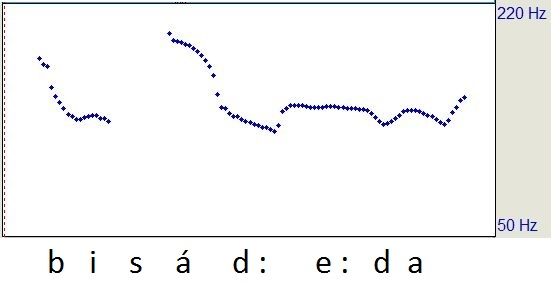
\includegraphics[width=5cm]{figures/downing-img1.jpg}
\caption{ \textit{bisáddeeda} ‘her cat’}
\label{fig:downing:1}
\end{figure}



Our data thus tends to confirm \citegen{Hyman1981} observation that the possessive undergoes accent (High tone) reduction, except that High tone reduction is variable in our corpus: it does not occur 100\% of the time.

Interestingly, our data shows that the likelihood of realization of the determiner’s High tone is construction specific. For example, the demonstrative suffixes also often lack a High tone: out of a total of 635 instances of Noun+de\-mon\-stra\-tive constructions in our corpus, 369 (58\%) do not realize a High tone on the demonstrative suffix. This variation is illustrated in \REF{ex:downing:7}:

\ea 
\label{ex:downing:7}
\ea  \textit{wíil-k}\textbf{\textit{a}}\textit{n}  ‘this boy’  (\textasciitilde\textit{wíil-k}\textbf{\textit{á}}\textit{n)}\\

\ex   \textit{gaarí-g}\textbf{\textit{aa}}\textit{s}  ‘that car’  (\textasciitilde\textit{gaarí-g}\textbf{\textit{aá}}\textit{s)}\\

\ex   \textit{Talaadá-d}\textbf{\textit{aa}}\textit{s}  ‘that Tuesday’  (\textasciitilde\textit{ Talaadá-d}\textbf{\textit{aá}}\textit{s)}\\
\z
\z

This is a significantly lower proportion of missing High tones, however, than found with the possessive suffixes.

In contrast, the remote definite suffix more generally realizes its High tone. Out of 997 instances of Noun+remote definite constructions in our corpus,\footnote{This set of 997 excludes constructions where the remote definite suffix occurs in a non-focused subject NP.} only 358 (36\%) do not realize a High tone on the remote definite suffix. This variation is illustrated in \REF{ex:downing:8}:


\ea \label{ex:downing:8}
\ea  \textit{mindí-di}\textbf{\textit{i}}  ‘that (remote) knife’  (\textasciitilde \textit{ mindí-di}\textbf{\textit{í}})\\
\ex   \textit{nín-ki}\textbf{\textit{i}}  ‘that (remote) man’  \textit{({\textasciitilde} nín-ki}\textbf{\textit{í}})\\
\ex   \textit{qoraallá-di}\textbf{\textit{i}}  ‘those (remote) texts’  (\textasciitilde \textit{ qoraallá-di}\textbf{\textit{í}})\\
\z
\z

Finally, Noun+modifier constructions should have a High tone assigned to the final syllable of the second word.\footnote{Nouns can be followed by more than one modifier, and it is the final modifier which should realize a final High tone. We consider here only nouns followed by a single modifier, for ease of comparison with the Noun+determiner data.} Yet, in our data, this High tone is again often missing. Out of 571 instances of Noun+indefinite Noun constructions in our corpus,\footnote{This number excludes feminine nouns – mostly personal names and place names – with a fixed (exceptional) accent on a non-final mora, which show much less variability in their tonal behavior.} 391 (68.5\%) do not realize a High tone on the second noun. This variation is illustrated in (\ref{ex:downing:9a}, \ref{ex:downing:9b}); recall that numbers are nouns in Somali. Out of 599 instances of Noun+Adjective constructions, in contrast, only 297 (50\%) do not realize a High tone on the modifier. This variation is illustrated in (\ref{ex:downing:9c}, \ref{ex:downing:9d}):\footnote{This set of 599 excludes constructions where the adjective either has the subject suffix \textit{-i} or has an exceptional, fixed penult accent (in our data: \textit{wéyn} ‘big’, \textit{dhéer} ‘long’, \textit{macáan} ‘sweet’), which show almost no variability in their tonal behavior.}\pagebreak


\ea \label{ex:downing:9}
\ea  \textit{hál} \textit{lit}\textbf{\textit{i}}\textit{r}  ‘one liter’  ({\textasciitilde} \textit{hál lit}\textbf{\textit{í}}\textit{r)}  \label{ex:downing:9a}\\
\ex   \textit{gúri-ga} \textit{Muus}\textbf{\textit{e}}  ‘Musa’s house’  ({\textasciitilde} \textit{gúri-ga Muus}\textbf{\textit{é}}) \label{ex:downing:9b}\\
\ex   \textit{biyó} \textit{bad}\textbf{\textit{a}}\textit{n}  ‘much water’  ({\textasciitilde} \textit{biyó bad}\textbf{\textit{á}}\textit{n)} \label{ex:downing:9c}\\
\ex   \textit{subáx-dií} \textit{hor}\textbf{\textit{e}}  ‘(in) the early morning’  ({\textasciitilde} \textit{subáx-dií hor}\textbf{\textit{é}}) \label{ex:downing:9d}\\
\z
\z

To sum up this section, High tones on determiners and nominal modifiers are often not realized. All the speakers exhibit the same range of variation, so it cannot be attributed to dialectal or individual differences. In the next section, we take up two untenable phonological accounts – the OCP and Final Lowering – for why these High tones are missing before arguing for an alternative analysis in \sectref{sec:downing:4}.


\section{Why the OCP and Final Lowering cannot account for the missing High tones}
\label{sec:downing:3}

\subsection{The OCP}


Looking at \figref{fig:downing:1}, above, one might propose that the High tone on the possessive suffix – and other determiners – is deleted as an OCP effect \citep{leben1973suprasegmental}: in a sequence of adjacent High tones, one is deleted. However, this explanation faces the problem that the OCP is not a general principle of the Somali tone system. When two consecutive High tones occur, they are normally realized on almost the same pitch level. This is illustrated in the pitch track for (\ref{ex:downing:9d}), \textit{subáxdií hore} ‘(in) the early morning’ given in \figref{fig:downing:2}.

  
\begin{figure}
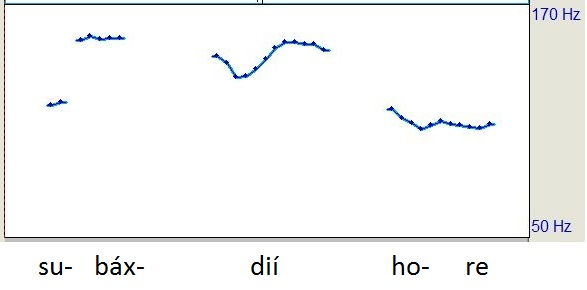
\includegraphics[width=5cm]{figures/downing-img2.jpg}
\caption{\textit{subáxdií hore} ‘(in) the early morning’}                
\label{fig:downing:2}
\end{figure}
 
Therefore, tonal reduction on possessives and other determiners is not plausibly motivated by the OCP. Furthermore, the OCP is not relevant in the case of the missing High tones on the final vowels of modifiers in Noun+modifier constructions, such as \textit{hore} ‘early’ in this example.

\subsection{Final Lowering}


The Somali tone literature \citep{Andrzejewski1981,Armstrong1934,Hyman1981,LeGac2003,Saeed1993,Saeed1999} notes that High tones are lowered phrase-finally\slash pre-pausally\slash post-focally. Since the ``missing'' High tones in our data – in both Noun+determiner and Noun+modifier constructions – often occur in phrase-final position, one might propose that Final Lowering is responsible for giving the impression that the High tones have been deleted. However, Final Lowering does not provide a general explanation for the missing High tones in our data. First, the expected High tone on the possessive suffix (e.g., \textit{dhég-}\textbf{\textit{tíisa}} ‘his ear’) is not associated with the final syllable or mora, so Final Lowering is not relevant here. Second, final High tones are not deleted in our data in other morphosyntactic contexts, such as lexical words in isolation \REF{ex:downing:10} and in sentence final position \REF{ex:downing:11}, where the final High tone is expected to be realized. Non-lowered final High-toned vowels are bolded:


\ea  Words in isolation  \label{ex:downing:10}
\ea  \textit{tukay}\textbf{\textit{aá}l}  ‘crows’ 
\ex   \textit{ubaxy}\textbf{\textit{ó}}  ‘flowers’ 
\ex   \textit{lafdhabarr}\textbf{\textit{ó}}  ‘spines’
\z
\z

\ea  Sentence final position \label{ex:downing:11}
\ea  \textit{Wáxaan arkay rat}\textbf{\textit{í}}.  ‘I saw a camel.’ 
\ex   \textit{Waxaan lá kulmay Sahr}\textbf{\textit{ó}}.  ‘I met with Sahra.’
\ex \textit{Hooyadáa waa macallim}\textbf{\textit{á}}\textit{d}.  ‘Your mother is a teacher.’
\ex \textit{Libáax ayáa dilaý dawac}\textbf{\textit{ó}}.  ‘A lion killed a fox.’
\z
\z

That is, final High tones are not systematically deleted. Only High tones on (some) postnominal determiners and modifiers are.

Third, High tones can be deleted from the word-final syllable of a determiner or a modifier even when the word is not phrase-final or pre-pausal:


\ea Vowels with ``missing'' non-final High tones are bolded \label{ex:downing:12}
\ea  \textit{labá} \textit{dúmar} \textit{ah} \textit{oo} \textit{qurúx} \textit{bad}\textbf{\textit{a}}\textit{n} \textit{oo} \textit{kalíya} \\
  ‘just two beautiful women’ (cf. \textit{labá} ‘two’; \textit{dúmar} ‘women’;   \textit{qurúx} ‘beauty’; \textit{bad}\textbf{\textit{á}}\textit{n} ‘much’; \textit{kalíya} ‘only’)\\
\ex   \textit{sánnad-k}\textbf{\textit{ii}} \textit{hore} \textit{{\textasciitilde} sánnad-k}\textbf{\textit{ií}} \textit{hore} \\
  ‘last year’ (cf. \textit{sánnad} ‘year’; \textit{horé} ‘previous’)\\
\ex   \textit{bisád-d}\textbf{\textit{aa}}\textit{s} \textit{yar} \textit{{\textasciitilde} bisád-d}\textbf{\textit{aá}}\textit{s} \textit{yar} \\
  ‘that little cat’ (cf. \textit{bisád} ‘cat’; \textit{yár} ‘small’)\\
\z
\z

To sum up this section, neither the OCP nor Final Lowering can account for the missing High tones in N+determiner and N+modifier constructions, because neither of these processes applies generally in Somali. Instead, High tone deletion\slash non-realization appears to be construction specific. Further, High tones are often deleted when the context for neither the OCP or Final Lowering is met.


\section{Tone ``deletion'' as prosodic restructuring}
\label{sec:downing:4}

\subsection{Parallels with Swedish prosody}


Coming from a Swedish background, one is struck by the similarities between the prosodic systems of Somali and Swedish, another language with a stress-like tone system. As argued for in recent work by \citet{Riad2012, Riad2016} and \citet{Myrberg2015}, Swedish has prosodic culminativity of stress at the PWord\textsubscript{(min)} level and culminativity of tone at the PWord\textsubscript{(max)} level; compounds are a single tone realization\slash assignment domain; and some affixes are stressed, while others are not. Data illustrating these properties for Swedish are given in \xxref{ex:downing:13}{ex:downing:15}; all of the data are cited from \citet{Myrberg2015}. In \REF{ex:downing:13}, we see that Swedish does not have secondary stress, unlike English or German:

\ea  PWord culminativity for stress \label{ex:downing:13}
\ea  American English and Swedish stress
\begin{xlist}
\ex  (ˈmoneˌtary)$_ω$  (moneˈtär)$_ω$min=max\\
\ex  (toˌtaliˈtarian)$_ω$  (totaliˈtär)$_ω$min=max\\
\ex  (ˈabˌstract)$_ω$  (abˈstrakt)$_ω$min=max\\
\end{xlist}
\ex  German and Swedish stress\\
\begin{xlist}
\ex  (ˌmiliˌtariˈsieren)$_ω$  (militariˈsera)$_ω$min=max\\
\ex  (ˌonoˌmatopoˈetisch)$_ω$  (onomatopoˈetisk)$_ω$min=max\\
\ex  (ˌuniˌversiˈtät)$_ω$  (universiˈtet)$_ω$min=max\\
\end{xlist}
\z
\z

The data in \REF{ex:downing:14} shows that compounds have two stresses but a single tonal accent (accent 2, indicated with a diacritic superscripted before the compound) realized over the entire compound and replacing the isolation tone pattern of the words making up the compound:


\ea  Compounds \label{ex:downing:14}
\ea  sommar-lov   $^2$((ˈsommar$_2$)$_ω$min(ˌlov$_1$)$_ω$min)$_ω$max \\
     ‘summer break’\\
\ex   jul-lovs-morgon  $^2$((ˈjul$_1$)$_ω$min(ˌlov$_1${}-s)$_ω$min(ˌmorgon$_2$)$_ω$min)$_ω$max \\
    ‘Christmas break morning’\\
\ex   jul-klapp   $^2$((ˈjul$_1$)$_ω$min(ˌklapp$_1$)$_ω$min)$_ω$max \\
     ‘Chistmas present’\\
\z
\z

The data in \REF{ex:downing:15} illustrates that some affixes bear a stress and takes part in the realization of a tonal accent 2 in the construction, while others –  \REF{ex:downing:15c} – bear neither stress nor tone:


\ea  Affixes \label{ex:downing:15}
\ea  tvätt-bar  $^2$((ˈtvätt)$_ω$min(ˌbar)$_ω$min)$_ω$max   ‘washable’ \textbf{tonic} \textbf{suffix} \label{ex:downing:15a}\\
\ex   o-nödig  $^2$((ˈo)$_ω$min(ˌnöd-ig)$_ω$min)$_ω$max   ‘unnecessary’ \textbf{tonic} \textbf{prefix}\label{ex:downing:15b}\\
\ex   för-ändra  (för-$^1$(ˈändra)$_ω$min)$_ω$max   ‘to change’\label{ex:downing:15c}\\
\z
\z

All of these properties also characterize Somali’s prosodic system, as we have seen in the preceding sections. \tabref{extab:downing:16} summarizes the similarities in the prosodic systems of the two languages.


\begin{table} 
\caption{Comparison of the prosody of Swedish and Somali\label{extab:downing:16}}
\begin{tabular}{lll} 
\lsptoprule
& Somali & Swedish\\
\midrule
PWord culminativity & \ding{52}\footnote{tone} & \ding{52}\footnote{stress (PWord\textsubscript{min}); tonal accent (PWord\textsubscript{max})}\\
compounds are 1 tone realization domain & \ding{52} & \ding{52}\\
stressable/tone bearing affixes & \ding{52} & \ding{52}\\
\lspbottomrule
\end{tabular}
\end{table}

\subsection{Prosodic restructuring in Swedish}


Another property the Swedish and Somali prosodic systems have in common is that a tone (accent) is obligatory. In Swedish, tonal accent is obligatory for all PWord\textsubscript{(max)}, and in Somali, for all nominals and modifiers when pronounced in isolation. Yet, in both languages, an expected High tone (or accent) is sometimes ``missing''. We illustrated the ``missing'' High tones of Somali in \sectref{sec:downing:3}. For Swedish, as work like \citet{Garlén1988,Myrberg2015} and \citet{Riad2016} reports, words in some short phrases, which sometimes are even structurally similar to those in our Somali data, variably lose their tonal accent. This phenomenon is illustrated in \REF{ex:downing:17}. As we can see in this data, the input tone-accent is sometimes simplified. Accent 2 can be reduced to accent 1 – as in \REF{ex:downing:17a}. The examples in \xxref{ex:downing:17b}{ex:downing:17c} illustrate that often only the accent of the rightmost PWord in the phrase is consistently realized. (In this data set, subscripted numbers indicate the input tonal accents. Superscripted numbers indicate the tonal accents realized under prosodic adjunction):
     
\ea  Prosodic restructuring in Swedish (\citealt{Myrberg2015}) \label{ex:downing:17}
\ea  Prosodic adjunction in morphology and syntax \label{ex:downing:17a}\\

  morphology:  (för-$^1$(ˈändra$_2$)$_ω$)$_ω$max   ‘to change’ \\

  syntax:  (för $^1$(ˈliten$_2$)$_ω$)$_ω$max  ‘too small’\\

      (för $^1$(ˈmånga$_2$)$_ω$)$_ω$max  ‘too many’\\

      (för $^1$(ˈlänge$_2$)$_ω$)$_ω$max  ‘too long’\\

\ex   Lexicalized phrases with prosodic adjunction\label{ex:downing:17b}\\

((ˈröd-a$_2$)$_ω$ $^2$(ˈmatt-an$_2$)$_ω$)$_ω$max  ‘red carpet’ (lexicalised phrase)\\

((ˈRöd-a$_2$)$_ω$ $^1$(ˈKors-et$_1$)$_ω$)$_ω$max   ‘Red Cross’ (name, lexicalised)\\

((ˈhopp-a$_2$)$_ω$ $^1$(ˈupp$_1$)$_ω$)$_ω$max  ‘jump up’  (particle verb)\\

((ˈhel-a$_2$)$_ω$ (ˈlång-a$_2$)$_ω$ $^1$(ˈdag-en$_1$)$_ω$)$_ω$max ‘all day, lit. whole long day’\\

\ex   Local deaccentuation as the result of prosodic adjunction\label{ex:downing:17c}\\

((ˈliten$_2$)$_ω$ $^2$(ˈsmuts-ig$_2$)$_ω$)$_ω$max $^2$(ˈgryt-a$_2$)$_ω$min=max  ‘little dirty pot’\\
                                                                                                                                       
((ˈlag-a$_2$)$_ω$ (be-$^1$(ˈgagn-ade$_2$)$_ω$)\textsubscript{ω’})$_ω$max (kopia$^1$ˈtorer$_1$)$_ω$min=max ‘repair used copying machines’\\
\z
\z     

{To account for this variation in output accent realization, \citet{Myrberg2015} and \citet{Riad2016} propose that both words and affixes can be incorporated into a single PWord\textsubscript{(max)} via prosodic restructuring (adjunction). (Their restructuring analysis is illustrated in the prosodic representations in \REF{ex:downing:17}.) Prosodic restructuring accounts for the tonal reduction found, given the culminative one tonal accent per PWord\textsubscript{(max)} principle which \citet{Riad2016} shows holds for Swedish. Reducing the number of PWord\textsubscript{(max)} in a phrase necessarily reduces the number of tonal accents that can be realized.}\\

\subsection{Prosodic restructuring in Somali}

What we propose is that Somali High tone reduction is the result of prosodic restructuring, analogous to what has been proposed for Swedish by \citet{Myrberg2015} and \citet{Riad2016} and illustrated in the preceding section. We also adopt from their analysis a distinction between PWord\textsubscript{(min)} and PWord\textsubscript{(max)}.\footnote{Following \citet{Myrberg2015} and \citet{Riad2016}, we adopt a distinction between PWord-min and PWord-max as defined in work like \citet{Ito2012, Ito2013}.} We follow work like \citet{Green2016,Hyman1981,Hyman2006, Hyman2012,LeGac2003} and \citet{Saeed2004} in assuming that a culminative one High tone per PWord principle holds for Somali. For High-toned determiners like the possessive to be realized with a High tone, we propose that they must therefore be parsed in a separate PWord\textsubscript{(min)} from the noun they modify. However, High-toned determiners are arguably parsed in the same PWord\textsubscript{(max)} domain as a preceding noun, because they undergo segmental sandhi processes which do not apply across PWord\textsubscript{(max)} boundaries. The representations in \REF{ex:downing:18} illustrate our analysis:\footnote{See \citet{Green2016} for an alternative account of similar Somali data. Space does not permit a careful critical comparison of our analysis with theirs. The interested reader is directed to their work for details.}

\ea \label{ex:downing:18}
\ea ((dhég)\textsubscript{PWord-min} (\textbf{t}íisa)\textsubscript{PWord-min})\textsubscript{PWord-max}   ‘his ear’ \label{ex:downing:18a}
\ex ((mindí)\textsubscript{PWord-min} (\textbf{d}íisa)\textsubscript{PWord-min})\textsubscript{PWord-max} ‘his knife’ \label{ex:downing:18b}
\z
\z

Note that the alternation between \textit{-diisa} and \textit{-tiisa} in \REF{ex:downing:18} is an example of a sandhi process that only applies across a PWord-min boundary within PWord-max in our analysis. (See \citealt[28--31]{Saeed1999} for detailed discussion of these segmental sandhi processes.)

In the variable pronunciation where the possessive, for example, has lost its High tone, we propose that the construction has the same recursive PWord structure as the toneless definite determiner suffix – cf. (\ref{ex:downing:5}a). That is, the construction has undergone prosodic restructuring like that found in Swedish \REF{ex:downing:17}, so that the possessive suffix is not an independent PWord\textsubscript{(min)}, but rather is adjoined to the preceding noun within PWord\textsubscript{(max)}, as shown in \REF{ex:downing:19} – cf.  \REF{ex:downing:18a} and \REF{ex:downing:19b}:

\ea \label{ex:downing:19}
\ea ((dhég)\textsubscript{PWord-min} ta)\textsubscript{PWord-max}   ‘the ear’ \label{ex:downing:19a}
\ex ((dhég)\textsubscript{PWord-min} tiisa)\textsubscript{PWord-max}   ‘his ear’ \label{ex:downing:19b}
\z
\z

Since High tone is culminative and obligatory within the PWord\textsubscript{(min)} domain, reducing the number of PWord\textsubscript{(min)} within a PWord\textsubscript{(max)} domain necessarily leads to a reduction in the number of High tones realized within PWord\textsubscript{(max)}.

We propose that Noun+modifier phrases that have ``lost'' the High tone on the modifier have a similar analysis. They also undergo prosodic restructuring, but they are parsed into a different prosodic domain from the restructured determiners. Following \citet{Vigário2010} and \citet{vogel2010phonology}, we assume a Complex Word Group (CWG) constituent, which is the domain of, for example, tone assignment to compounds. Recall from \REF{ex:downing:1c}, above, that compounds in Somali form a single tonal realization domain; more examples are given in \REF{ex:downing:20}:

\ea \label{ex:downing:20}
\ea  \textit{madax-weýn-e} (m.) ‘president’ (cf. \textit{mádax} (m.) ‘head’; \textit{wéyn} ‘big’; \textit{{}-e} agentive suff.)\\
\ex   \textit{cod-kác} (m.) ‘tonal accent’ (cf. \textit{cód} (m.) ‘voice’; \textit{kac-} ‘rise’)\\
\ex   \textit{biya-dhác} (m.) ‘waterfall’ (cf. \textit{biyó} (pl.) ‘water’; \textit{dhac-} ‘fall’)\\
\ex   \textit{bad-wéyn} (f.) ‘ocean’ (cf. \textit{bád} (f.) ‘sea’; \textit{wéyn} ‘big’)\\
\ex   \textit{magaala-mádax} (f.) ‘capital’ (cf. \textit{magaálo} (f.) ‘town’; \textit{mádax} (m.) ‘head’)\\
\ex   \textit{laf-dhábar} (f.) ‘spine’ (cf. \textit{láf} (f.) `bone'; \textit{dhábar} (m.) ‘back’) \\
\z
\z

We propose that restructured Noun+modifier phrases are also parsed into a CWG, as illustrated in \REF{ex:downing:21} – cf. (\ref{ex:downing:5}d), above:

\ea  ((hál)\textsubscript{PWord-max} litir)\textsubscript{CWG} ‘one liter’ \label{ex:downing:21}
\z

It is interesting to note that tonal reduction results in a High tone on the leftmost word of the Noun+modifier construction, whereas compounding typically results in a single High tone on the rightmost word. We conclude that these two constructions must have a different prosodic representation. As illustrated in \REF{ex:downing:22}, prosodic restructuring of a Noun+modifier leads to a left-headed construction, whereas compounds are right headed:\footnote{A reviewer notes that another difference between restructured N+modifier phrases and compounds is that the tonal accent (and prosodic structure) assigned to compounds never varies. We propose that the lack of variation in compounds is due to the fact that they are lexicalized forms, morphosyntactically non-compositional. High tone variation in our data is found in compositional forms.}

\ea \label{ex:downing:22}
 prosodic restructuring: ((hál)\textsubscript{PWord-max} litir)\textsubscript{CWG} ‘one liter’\\

{vs.}\\

{compound:   (cod (kác)\textsubscript{PWord-max})\textsubscript{CWG} ‘tonal accent’}\\
\z

Both CWG constructions are posited to contain a PWord-max in order to account for the fact that segmental sandhi processes do not occur across the words in the CWG domain:


\ea  No segmental sandhi in the CWG domain \label{ex:downing:23}

prosodic restructuring:\\((labá)\textsubscript{PWord-max} tuug)\textsubscript{CWG}  (*labá duug) \textup{‘two thieves’}\\

vs. compound:\\   (keli (tális)\textsubscript{PWord-max})\textsubscript{CWG}  (* keli dális)  ‘dictatorship’\\
\textup{(cf.} \textup{kéli} (m.) ‘being alone’; \textup{tális} ‘government’)
\z

To account for tone assignment in these constructions, we propose that, in nominal CWGs, the High tone assigned to a CWG is realized on the internal PWord\textsubscript{(max)}. This is again analogous to Swedish, which only allows one tonal accent to be assigned both to a compound or compound-like construction, as well as to a construction that has undergone prosodic restructuring. The accent assignment principles for compounds and restructured words and phrases are not identical in Swedish. Note that this also generally holds true for Somali.

One last point in favor of our analysis is that it accounts for why determiners are added only to the rightmost word in a compound, whereas each noun in a Noun+Noun construction can have its own determiner, as shown in \REF{ex:downing:24}.


\ea \label{ex:downing:24}
    \begin{tabular}[t]{@{}lll@{}}
    & compound       &   Noun+Noun\\
a. & \textit{guri-márti-ga} ‘the guesthouse’ &  \textit{gúri-ga} \textit{martí-da} ‘the guests’ house’\\
b. & \textit{caana-géel-a} ‘the camel milk’  & \textit{caaná-ha} \textit{géel-a} ‘the camels’ milk’\\
\end{tabular}
\z

Recall that compounds and Noun+Noun constructions are also potentially distinguished by tone, as shown in \REF{ex:downing:24}. Noun+Noun constructions can have two High tones, one for each PWord, when they are not restructured, while compounds, which contain only one PWord, only have one High tone:

\ea\label{ex:downing:25}
\begin{tabular}[t]{@{}l>{\raggedright}p{4.5cm}l>{\raggedright\arraybackslash}p{4.5cm}@{}}
 & compound & &  Noun+Noun\\
a.& (guri(márti)\textsubscript{PWord-max})\textsubscript{CWG} ‘guesthouse’  & b. & (gúri)\textsubscript{PWord-max} (martí)\textsubscript{PWord-max} {\textasciitilde} ((gúri)\textsubscript{PWord-max} marti)\textsubscript{CWG} ‘guests’ house’ (cf. \textit{gúri} ‘house’; \textit{martí} ‘guests’)\\
c.& (caana(géel)\textsubscript{PWord-max})\textsubscript{CWG}  ‘camel milk’ & d. & (caanó)\textsubscript{PWord-max} (geél)\textsubscript{PWord-max} {\textasciitilde} ((caanó)\textsubscript{PWord-max} geel)\textsubscript{CWG} ‘camels’ milk’ (cf. \textit{caanó} ‘milk’; \textit{géel} ‘camels’)\\
\end{tabular}
\z 

We propose that a determiner takes a PWord as its base. Since compounds contain only one PWord, as shown in (\ref{ex:downing:25}a,\,c), they can take only one determiner. However, each noun in a Noun+Noun construction can be parsed as a PWord, as shown in (\ref{ex:downing:25}b, d), and so each can take a determiner. Strikingly, Noun1-determiner+Noun2-determiner constructions cannot be restructured; the High tone of the second noun is always realized. The determiner, which requires a PWord base, appears to block tonal reduction in Noun2. In our analysis, this falls out from proposing that both the determiner and the High tone require a PWord base. When Noun2 is not parsed as a PWord, under restructuring (see \ref{ex:downing:26}d), it can bear neither a determiner nor a High tone.

Our analysis is summarized schematically below (cf. \ref{ex:downing:5}, above); ‘X’ in compounds indicates that compounds can be made up of a combination of lexical words (X):


\ea Summary of our analysis  \label{ex:downing:26}
\ea N+definite:        ((N)\textsubscript{PWord-min} def)\textsubscript{PWord-max}
\ex N+H-toned determiner:  ((N)\textsubscript{PWord-min} (Det)\textsubscript{PWord-min})\textsubscript{PWord-max} 

  ~~ OR restructured    ((N)\textsubscript{PWord-min} Det)\textsubscript{PWord-max}
\ex compound:        (X (X)\textsubscript{PWord-max})\textsubscript{CWG}
\ex N+modifier:        (N)\textsubscript{ PWord-max} (Modif)\textsubscript{PWord-max} 

  ~~ OR restructured    ((N)\textsubscript{PWord-max} Modif)\textsubscript{CWG}
\z
\z


\section{Conclusion and topics for future research}

\label{sec:downing:5}
Many nominal constructions in Somali do not realize the expected High tones on the determiner or modifier; that is, they undergo tonal reduction. We argue that tonal reduction in Somali is the consequence of prosodic restructuring, rather than as the result of tone deletion or tonal lowering processes. Since High tone is culminative within the PWord\textsubscript{(min)} domain, prosodic restructuring which reduces the number of PWord\textsubscript{(min)} automatically reduces the number of High tones which can be realized in the domain. It is striking that prosodic restructuring in Somali so closely parallels prosodic restructuring in Swedish. This leads us to propose that restructuring is typical of these kinds of tonal systems: i.e., with tonal culminativity within a prosodic domain. An important question for future research is whether Somali High tones are underlying or assigned to PWord\textsubscript{(min)} (depending on morphosyntactic information, à la \citealt{Hyman1981}). While our analysis shows that High tone realization is conditioned by prosodic domain structure, the source of the High tones in the representation requires further investigation. 


\section*{Acknowledgements}
We thank our Somali language consultants for their patience in teaching us about their language. We are grateful to to Nina Hagen Kaldhol, two anonymous reviewers and a proofreader for thoughtful comments. We thank the ACAL audience for helpful feedback. We would like to acknowledge a grant from the Swedish Science Foundation (Vetenskapsrådet) which supports our research on Somali prosody. 


{\sloppy
\printbibliography[heading=subbibliography,notkeyword=this] 
}
\end{document}
